\subsubsection*{3.1.4.}
设 $(V_1,T_1)$ 是在 $(V,T)$ 上添加领圈所得：
\[
V_1-V^\circ\simeq\partial V\times[0,1],
\qquad
T_1|_{V_1-V^\circ}=\operatorname{id}.
\]
定义如下 $D_t$ 上的空间（参见 1.4.3）：
\[
f':W\longrightarrow D_t.
\]

\begin{enumerate}[label=(\alph*)]
\item 设 $\widetilde D_t^*$ 是以 $y$ 为基点的 $D_t^*$ 的万有覆盖，并设 $W^*$ 为 $D_t^*$ 上的丛，它由 $V_1\times\widetilde D_t^*$ 对下述关系生成的等价关系取商而得：
\[
  (v,y)\sim(T_1v,e^{2\pi i}y).
  \]
\EditorialFootnote{这里 $y$ 位于万有覆盖，$e^{2\pi i}y$ 表示绕原点一周对应的覆盖变换，不能按复平面中乘以数值 $e^{2\pi i}=1$ 来解释。采用的是 1.1.5 的覆盖变换约定。}
\item 由于 $T_1|_{V_1-V^\circ}$ 平凡，可将 $W^*$ 与 $D_t$ 上以 $V_1-V$ 为纤维的平凡丛粘合，得到 $D_t$ 上的空间 $W_1$。
\item 令 $W=W_1\cup\{0\}$ 及 $f'(0)=0$。在 $W$ 上赋予唯一的拓扑，使其诱导 $W_1$ 的拓扑，使 $f'$ 连续，并且对 $t'<t$，${f'}^{-1}(\overline D_{t'})$ 为
$W_1\cap {f'}^{-1}(\overline D_{t'})$
的单点紧化。
\end{enumerate}

赋予 $W-\{0\}$ 以 1.3.4 中的可积联络，使 (a) 所给的 $W$ 在 $\widetilde D^*$ 上的逆像的平凡化为水平的。

\subsubsection*{命题 3.1.5.}
存在同胚
\[
\Psi:B_{t,d}\xrightarrow{\ \sim\ }W
\]
与到 $D_t$ 的投影相容，并将 $0$ 映至 $0$；可选择此同胚使其在 $0$ 之外为微分同胚。

本讨论班后续不会用到这一结果。

设 $d_0<d_1\leq r$，$t_0\leq\tau(d_0)$，并设 $y\in D_{t_0}^*$。有
\[
B_{t_0,d_0}\subset B_{t_0,d_1},
\]
且 $B_{t_0,d_1}-B_{t_0,d_0}^{\circ}$ 是 $D_{t_0}$ 上的丛。将其平凡化，并在圆周 $S_{|y|}$ 上，提升 $\partial/\partial\theta$，使与此平凡化相容。设 $T_1$ 是
\[
V_1=f^{-1}(y)\cap B_{t_0,d_1},
\qquad
V_0=f^{-1}(y)\cap B_{t_0,d_0}.
\]
的相应自同态。于是 $(V_0\subset V_1,T_1)$ 同构于 3.1.4 中的 $(V\subset V_1,T_1)$。设 $W$ 由 $(V_0\subset V_1,T_1)$ 构造。典范地有 ${f'}^{-1}(y)=V_1$。证明将表明可选择 $\Psi$，使其诱导恒等映射
\[
f^{-1}(y)\xrightarrow{\ \sim\ }{f'}^{-1}(y).
\]

下列 $f$ 及其在 $f^{-1}(\mathbb R)$ 上的限制的图示概括了证明。

\begin{center}
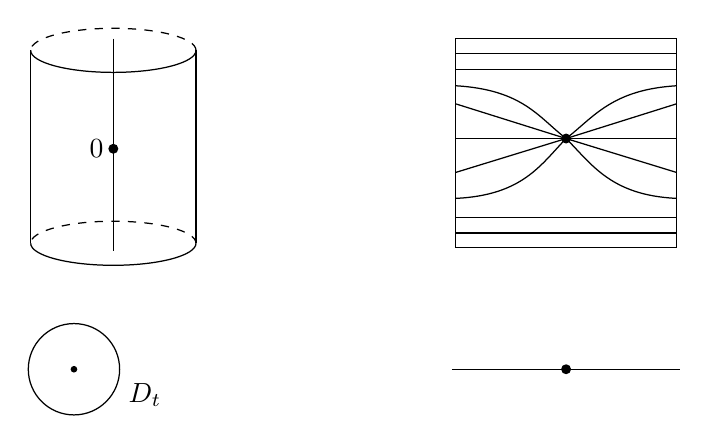
\begin{tikzpicture}[x=1cm,y=1cm,line width=.45pt]
  % Total space and base disc.
  \draw (-4.2,2.6) arc[start angle=180,end angle=360,x radius=1.05,y radius=.28];
  \draw[dashed] (-2.1,2.6) arc[start angle=0,end angle=180,x radius=1.05,y radius=.28];
  \draw (-4.2,2.6)--(-4.2,.15);
  \draw (-2.1,2.6)--(-2.1,.15);
  \draw (-4.2,.15) arc[start angle=180,end angle=360,x radius=1.05,y radius=.28];
  \draw[dashed] (-2.1,.15) arc[start angle=0,end angle=180,x radius=1.05,y radius=.28];
  \draw (-3.15,2.75)--(-3.15,.05);
  \fill (-3.15,1.35) circle (1.8pt);
  \node[left] at (-3.15,1.35) {$0$};
  \draw (-3.65,-1.45) circle (.58);
  \fill (-3.65,-1.45) circle (1.2pt);
  \node[right] at (-3.08,-1.78) {$D_t$};

  % Real slice and its base.
  \draw (1.2,.1) rectangle (4.0,2.75);
  \foreach \yy in {.28,.48,2.36,2.56}{\draw (1.2,\yy)--(4.0,\yy);}
  \draw (1.2,2.15) .. controls (2.05,2.10) and (2.25,1.75) .. (2.60,1.48)
                    .. controls (2.95,1.75) and (3.18,2.10) .. (4.0,2.15);
  \draw (1.2,.72) .. controls (2.05,.76) and (2.28,1.15) .. (2.60,1.48)
                   .. controls (2.93,1.15) and (3.17,.76) .. (4.0,.72);
  \draw (1.2,1.92)--(2.60,1.48)--(4.0,1.92);
  \draw (1.2,1.05)--(2.60,1.48)--(4.0,1.05);
  \draw (1.2,1.48)--(4.0,1.48);
  \fill (2.60,1.48) circle (1.8pt);
  \draw (1.15,-1.45)--(4.05,-1.45);
  \fill (2.60,-1.45) circle (1.8pt);
\end{tikzpicture}
\end{center}

设 $B^+\subset B_{t_0,d_1}$ 是满足
\[
|f(x)|^2\leq\tau(\delta(x)).
\]
的点 $x$ 所构成的集合。设 $\varphi_n$ 为从 $[0,t_0]$ 到 $(0,d_1]$ 的一列 $C^\infty$ 函数，使对某个趋于 $0$ 的序列 $t_0>r_1>r_2>\cdots$，

\begin{enumerate}[label=(\alph*)]
\item 对 $|t|^2\geq r_i$，$\varphi_i$ 是 $\tau$ 的反函数；
\item 对 $|t|^2<r_i$ 及 $j>i$，$\varphi_j(t)<\varphi_i(t)$。
\end{enumerate}

\begin{center}
\begin{tikzpicture}[x=1cm,y=1cm,>=Latex,line width=.5pt]
  \draw[->] (0,0)--(4.5,0) node[right] {$t$};
  \draw[->] (0,0)--(0,3.4) node[above] {$d$};
  \draw (0,3.0)--(3.05,3.0)--(3.05,0);
  \node[left] at (0,3.0) {$d_1$};
  \node[below] at (3.05,0) {$t_0$};
  \draw (0,0) .. controls (.35,1.05) and (1.35,2.15) .. (3.05,2.45);
  \node[right] at (3.05,2.45) {$t=\tau(d)$};
  \draw (0,1.45) .. controls (.45,1.42) and (.80,1.40) .. (1.18,1.68)
        .. controls (1.45,1.88) and (1.68,2.00) .. (1.92,2.10);
  \node at (.55,1.72) {$\varphi_0$};
  \draw (0,.58) .. controls (.23,.56) and (.35,.65) .. (.50,.90)
        .. controls (.67,1.18) and (.84,1.40) .. (1.18,1.68);
\end{tikzpicture}
\end{center}

空间 $B^+-\{0\}$ 是 $D_t$ 上由
\[
\delta(x)\geq\varphi_i(|f(x)|^2).
\]
所定义的丛 $B_i^+$ 的并。利用 $\delta$ 在 $B^+-\{0\}\to D_t$ 的各纤维上无临界点这一事实，标准论证表明：存在与到 $D_t$ 的投影相容的微分同胚 $\alpha_i:B_i^+\to B_{i+1}^+$，在 $B_i^+$ 的子空间
\[
\delta(x)=\varphi_i(|f(x)|^2),
\qquad |f(x)|^2\leq r_i,
\]
的一个小邻域之外等于恒等映射。复合各 $\alpha_i$ 并取极限，得到微分同胚
\[
\alpha:B_0^+-\{x\mid f(x)=0,\ \delta(x)=\varphi_0(0)\}
\xrightarrow{\ \sim\ }B^+-\{0\}.
\]
通过 $\alpha$ 搬运 $D_t$ 上丛 $B_0^+$ 的一个平凡化，得到 $B^+-\{0\}$ 上的可积联络 $\nabla'$。于是可以：

\begin{enumerate}[label=(\alph*)]
\item 将此联络在 $f^{-1}(S_{|y|})\cap B^+$ 上的限制延拓为 $f^{-1}(S_{|y|})/S_{|y|}$ 上的联络；此延拓给出 $T_1$；
\item 将 $\nabla'$ 在 $B^+-\{0\}$ 上给出的 $D_t$ 上径向向量场的提升，延拓至 $B_{t_0,d_1}$。
\end{enumerate}

于是，存在 $B_{t_0,d_1}$ 上唯一的可积联络 $\nabla$，延拓 $\nabla'$、(a) 和 (b)；并存在从 $B_{t_0,d_1}-\{0\}$ 到 $W-\{0\}$ 的唯一水平微分同胚，它在 $f^{-1}(y)$ 上为恒等。这就是所求的微分同胚。

